\begin{figure*}[!p]
    \centering
    \begin{minipage}[t]{0.48\textwidth}
        \centering
        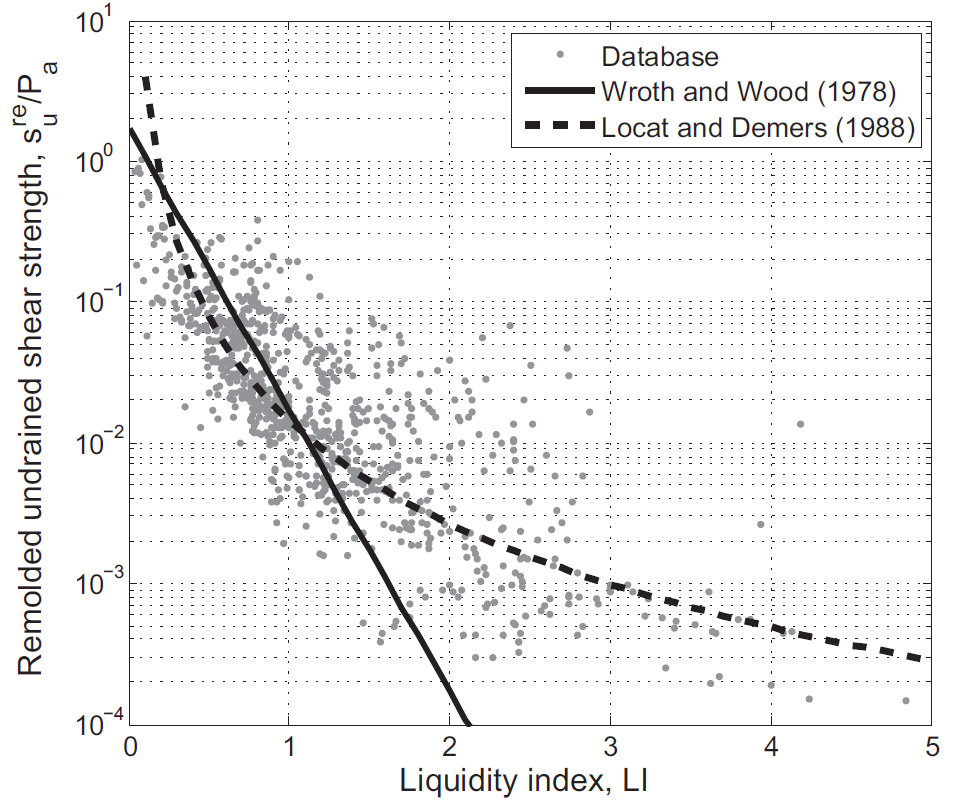
\includegraphics[width=\textwidth]{figures/figure-2.png}
        \caption{$\rm{LI}-(s_u^{re}/P_a)$ models proposed by \citet{Wroth1978137} and \citet{Locat1988799}.}
        \vspace{-5pt}
        \addtocounter{figure}{-1}
        \renewcommand{\figurename}{图}
        \caption{\citet{Wroth1978137}和\citet{Locat1988799}提出的$\rm{LI}-(s_u^{re}/P_a)$模型。}
        \label{figure:2}
        \renewcommand{\figurename}{Figure}
    \end{minipage}
    \begin{minipage}[t]{0.48\textwidth}
        \centering
        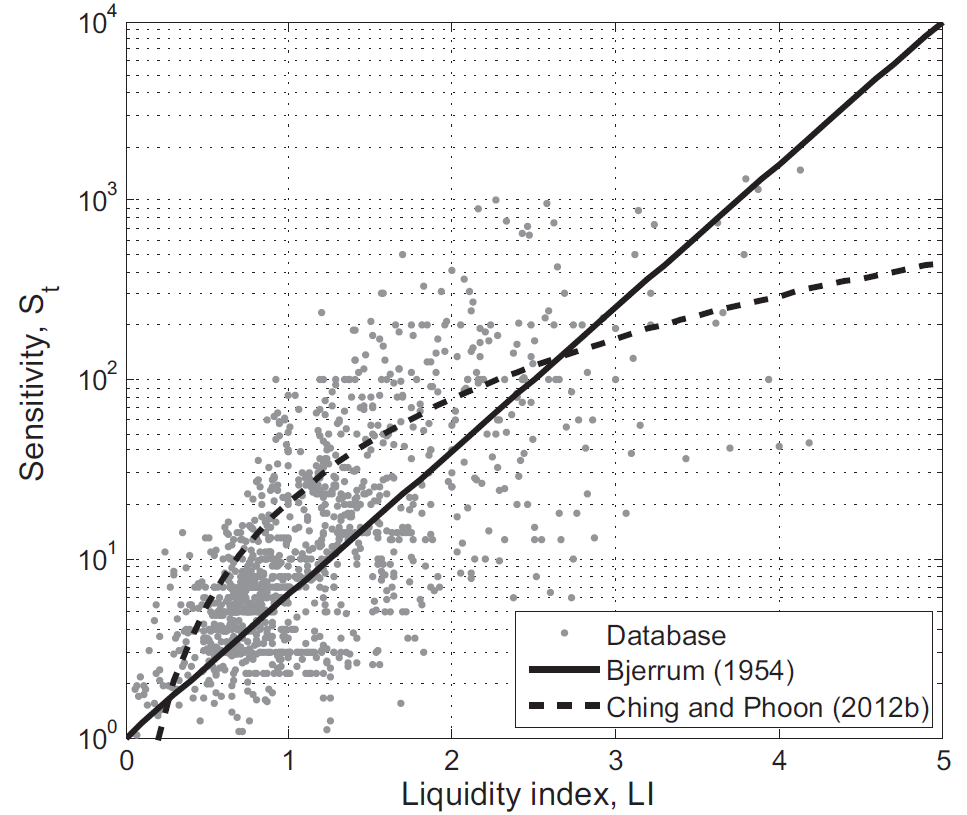
\includegraphics[width=\textwidth]{figures/figure-3.png}
        \caption{$\rm{LI}-S_t$ models proposed by \citet{Bjerrum195449} and \citet{Ching2012522}.}
        \vspace{-5pt}
        \addtocounter{figure}{-1}
        \renewcommand{\figurename}{图}
        \caption{\citet{Bjerrum195449}和\citet{Ching2012522}提出的$\rm{LI}-S_t$模型。}
        \label{figure:3}
        \renewcommand{\figurename}{Figure}
    \end{minipage}
\end{figure*}

\begin{figure*}[!p]
    \centering
    \begin{minipage}[t]{0.48\textwidth}
        \centering
        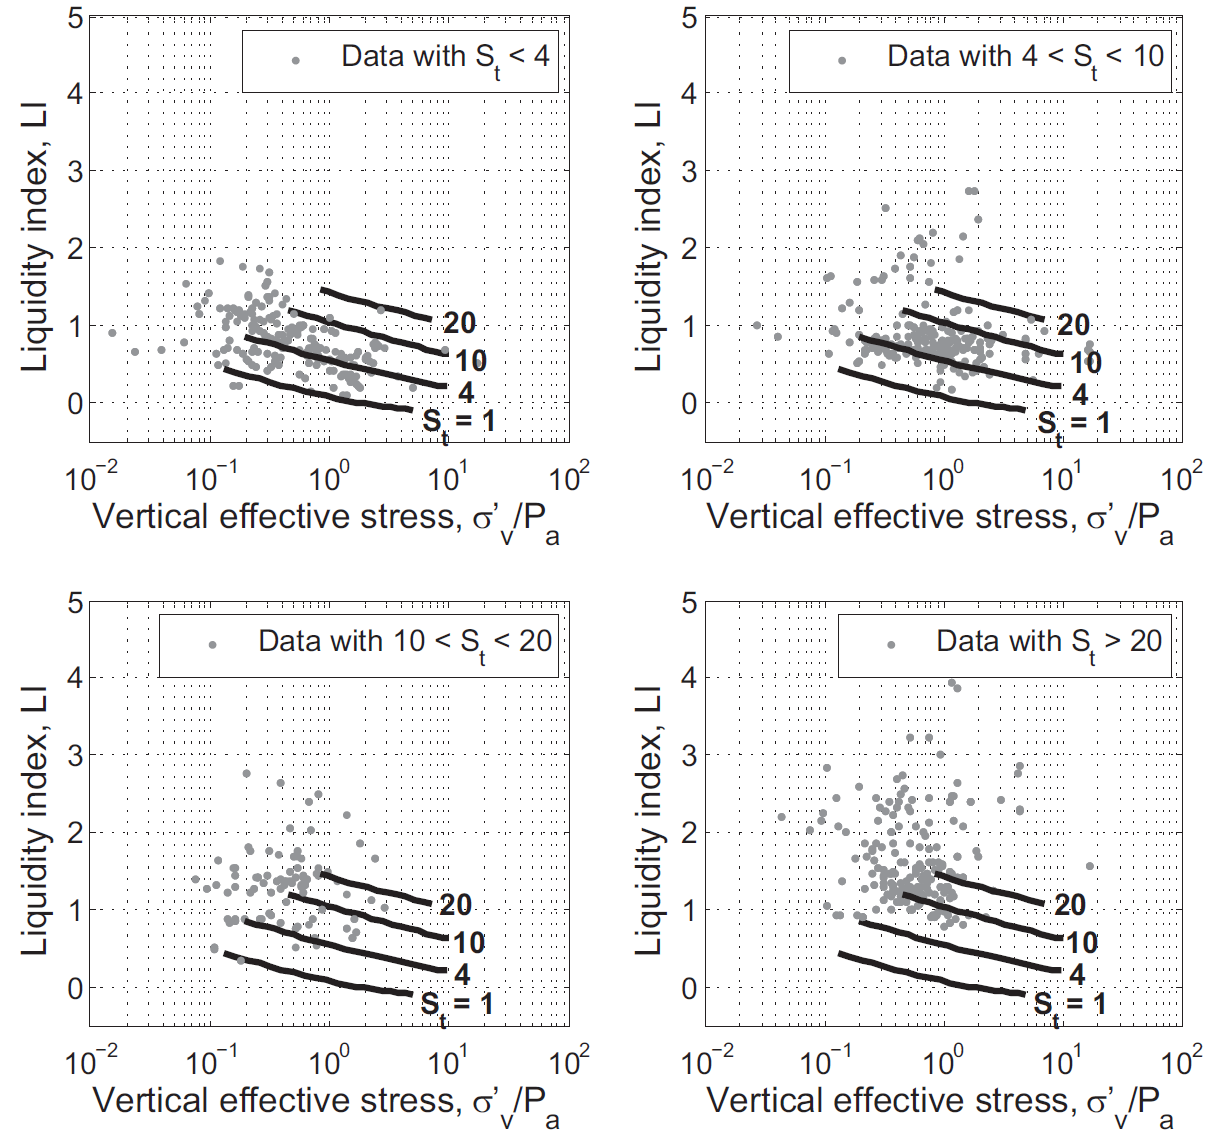
\includegraphics[width=\textwidth]{figures/figure-4.png}
        \caption{$\rm{LI}-(\sigma_v'/P_a)-S_t$ model proposed by \citet{Mitchell1993}.}
        \vspace{-5pt}
        \addtocounter{figure}{-1}
        \renewcommand{\figurename}{图}
        \caption{\citet{Mitchell1993}提出的$\rm{LI}-(\sigma_v'/P_a)-S_t$模型。}
        \label{figure:4}
        \renewcommand{\figurename}{Figure}
    \end{minipage}
    \begin{minipage}[t]{0.48\textwidth}
        \centering
        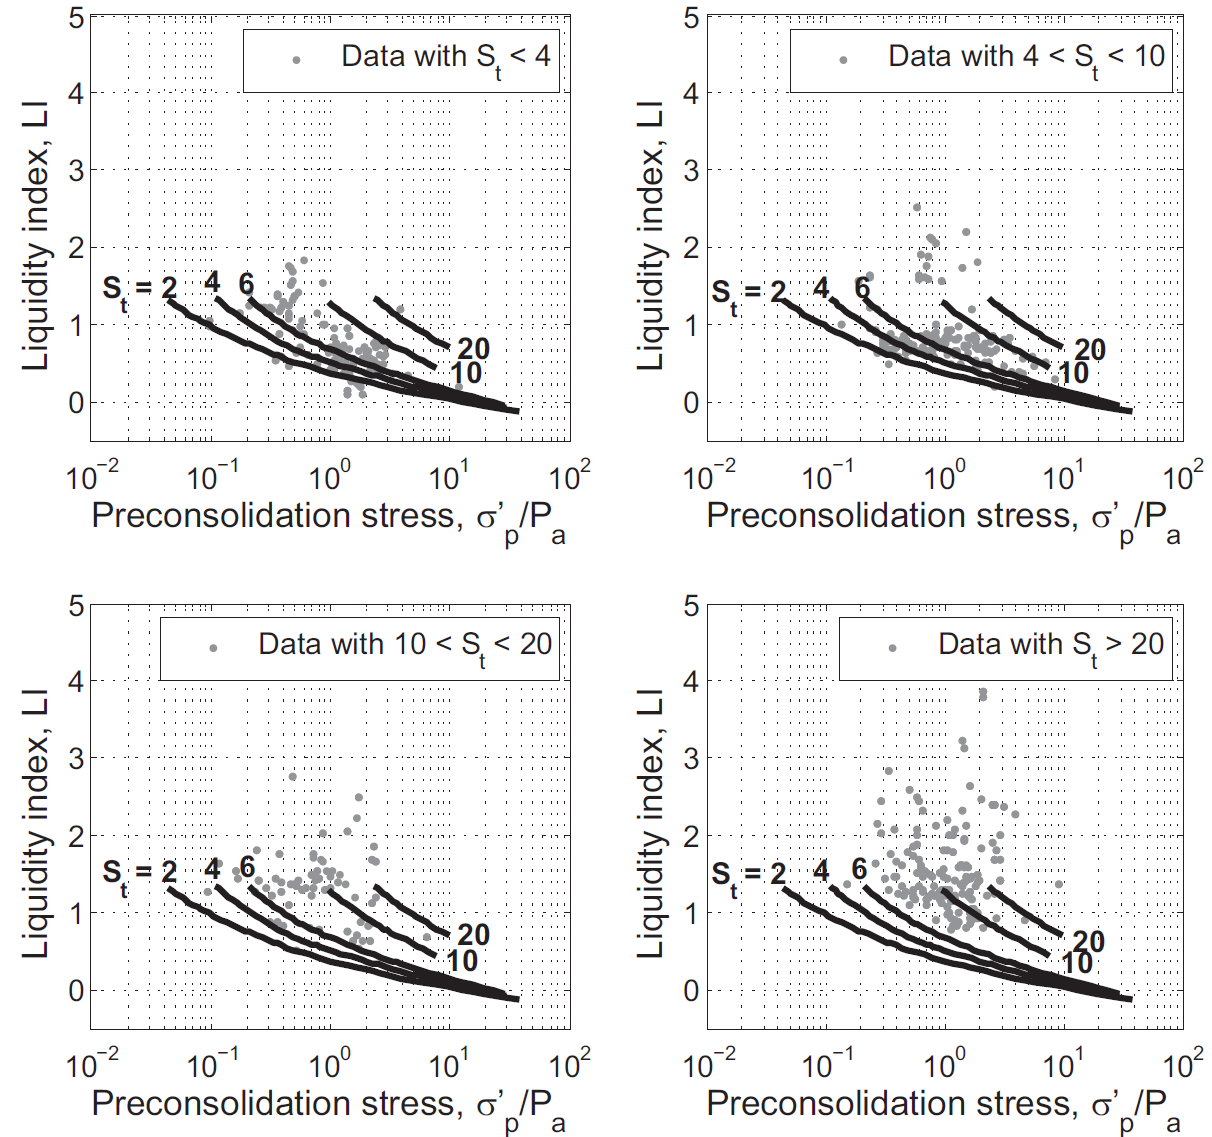
\includegraphics[width=\textwidth]{figures/figure-5.png}
        \caption{$\rm{LI}-(\sigma_p'/P_a)-S_t$ models proposed by \citet{NAVFAC1982}.}
        \vspace{-5pt}
        \addtocounter{figure}{-1}
        \renewcommand{\figurename}{图}
        \caption{\citet{NAVFAC1982}提出的$\rm{LI}-(\sigma_p'/P_a)-S_t$模型。}
        \label{figure:5}
        \renewcommand{\figurename}{Figure}
    \end{minipage}
\end{figure*}

\begin{figure*}[!p]
    \centering
    \begin{minipage}[t]{0.48\textwidth}
        \centering
        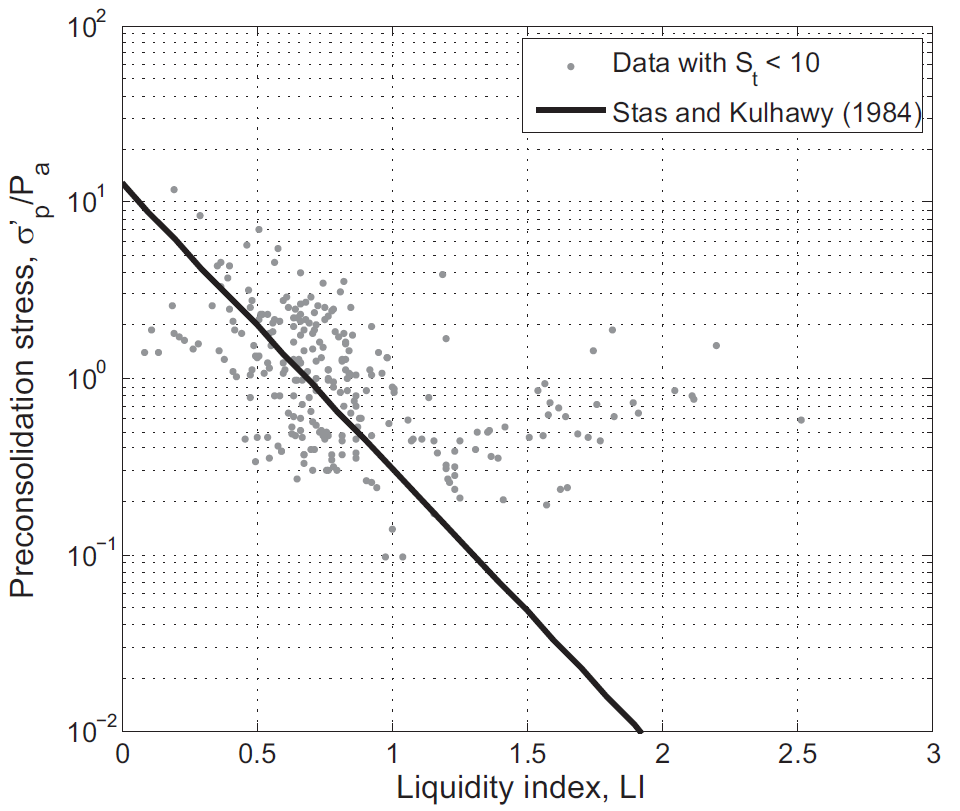
\includegraphics[width=\textwidth]{figures/figure-6.png}
        \caption{$\rm{LI}-(\sigma_p'/P_a)-S_t$ model proposed by \citet{Stas1984}.}
        \vspace{-5pt}
        \addtocounter{figure}{-1}
        \renewcommand{\figurename}{图}
        \caption{\citet{Stas1984}提出的$\rm{LI}-(\sigma_p'/P_a)-S_t$模型。}
        \label{figure:6}
        \renewcommand{\figurename}{Figure}
    \end{minipage}
    \begin{minipage}[t]{0.48\textwidth}
        \centering
        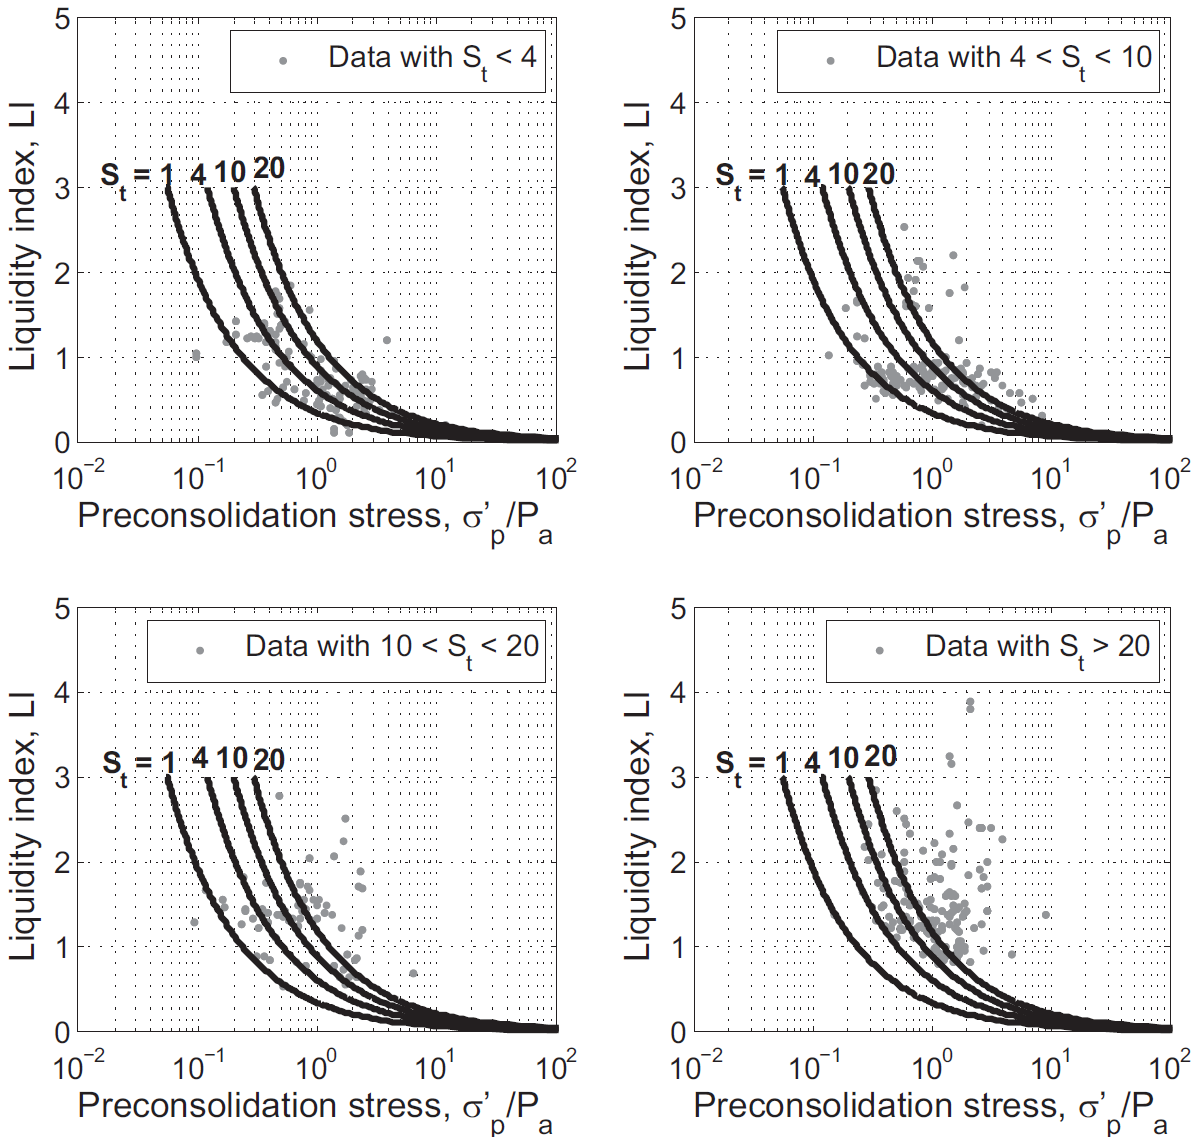
\includegraphics[width=\textwidth]{figures/figure-7.png}
        \caption{$\rm{LI}-(\sigma_p'/P_a)-S_t$ models proposed by \citet{Ching2012522}.}
        \vspace{-5pt}
        \addtocounter{figure}{-1}
        \renewcommand{\figurename}{图}
        \caption{\citet{Ching2012522}提出的$\rm{LI}-(\sigma_p'/P_a)-S_t$模型。}
        \label{figure:7}
        \renewcommand{\figurename}{Figure}
    \end{minipage}
\end{figure*}

\begin{figure*}[!p]
    \centering
    \begin{minipage}[t]{0.48\textwidth}
        \centering
        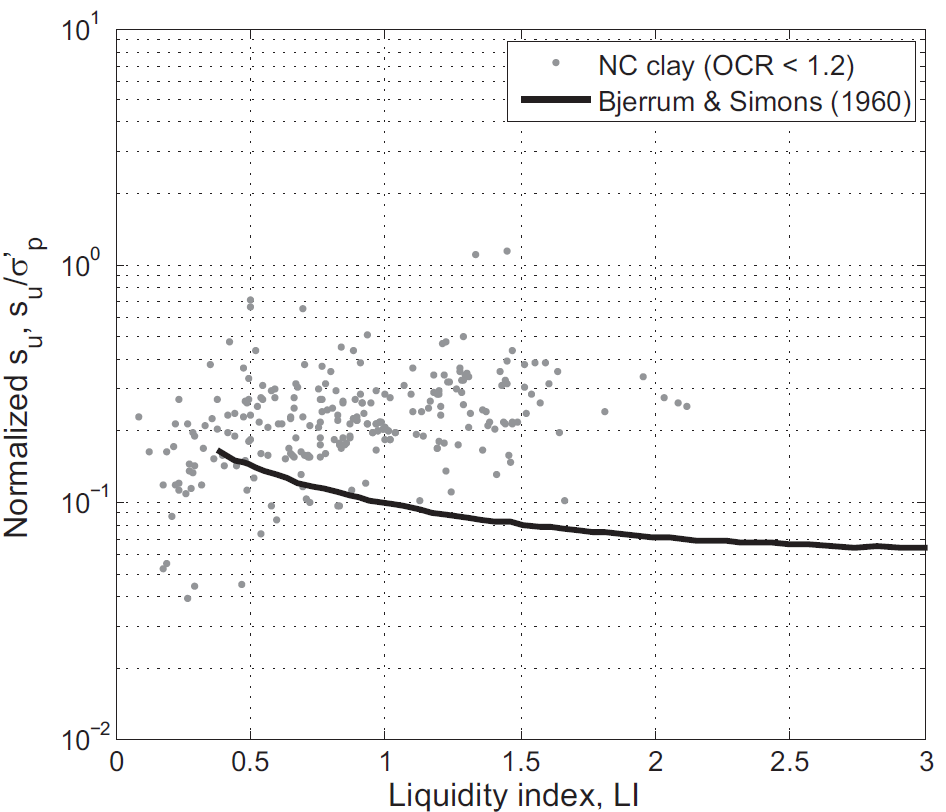
\includegraphics[width=\textwidth]{figures/figure-8.png}
        \caption{$\rm{LI}-(s_u/\sigma_p')$ model proposed by \citet{Bjerrum1960711}.}
        \vspace{-5pt}
        \addtocounter{figure}{-1}
        \renewcommand{\figurename}{图}
        \caption{\citet{Bjerrum1960711}提出的$\rm{LI}-(s_u/\sigma_p')$模型。}
        \label{figure:8}
        \renewcommand{\figurename}{Figure}
    \end{minipage}
    \begin{minipage}[t]{0.48\textwidth}
        \centering
        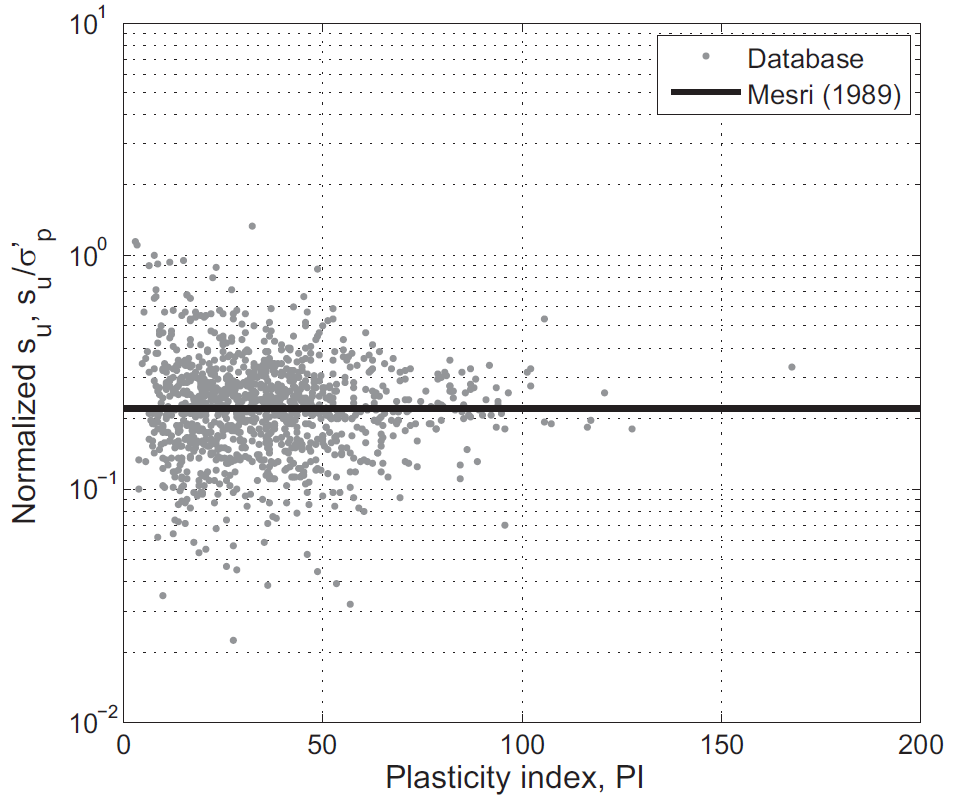
\includegraphics[width=\textwidth]{figures/figure-9.png}
        \caption{$\rm{LI}-(s_u/\sigma_p')$ models proposed by \citet{Mesri1975409, Mesri1989162}.}
        \vspace{-5pt}
        \addtocounter{figure}{-1}
        \renewcommand{\figurename}{图}
        \caption{\citet{Mesri1975409, Mesri1989162}提出的$\rm{LI}-(s_u/\sigma_p')$模型。}
        \label{figure:9}
        \renewcommand{\figurename}{Figure}
    \end{minipage}
\end{figure*}

\begin{figure*}[!p]
    \centering
    \begin{minipage}[t]{0.48\textwidth}
        \centering
        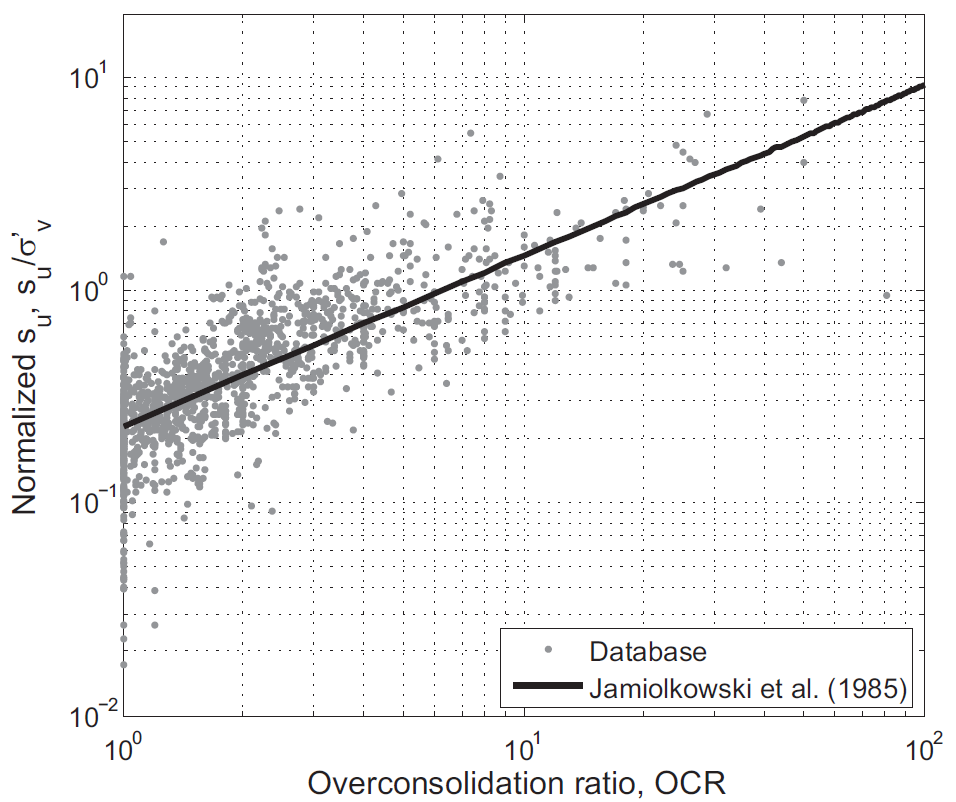
\includegraphics[width=\textwidth]{figures/figure-10.png}
        \caption{$\rm{OCR}-(s_u/\sigma_p')$ model proposed by \citet{Jamiolkowski198557}.}
        \vspace{-5pt}
        \addtocounter{figure}{-1}
        \renewcommand{\figurename}{图}
        \caption{\citet{Jamiolkowski198557}提出的$\rm{OCR}-(s_u/\sigma_p')$模型。}
        \label{figure:10}
        \renewcommand{\figurename}{Figure}
    \end{minipage}
    \begin{minipage}[t]{0.48\textwidth}
        \centering
        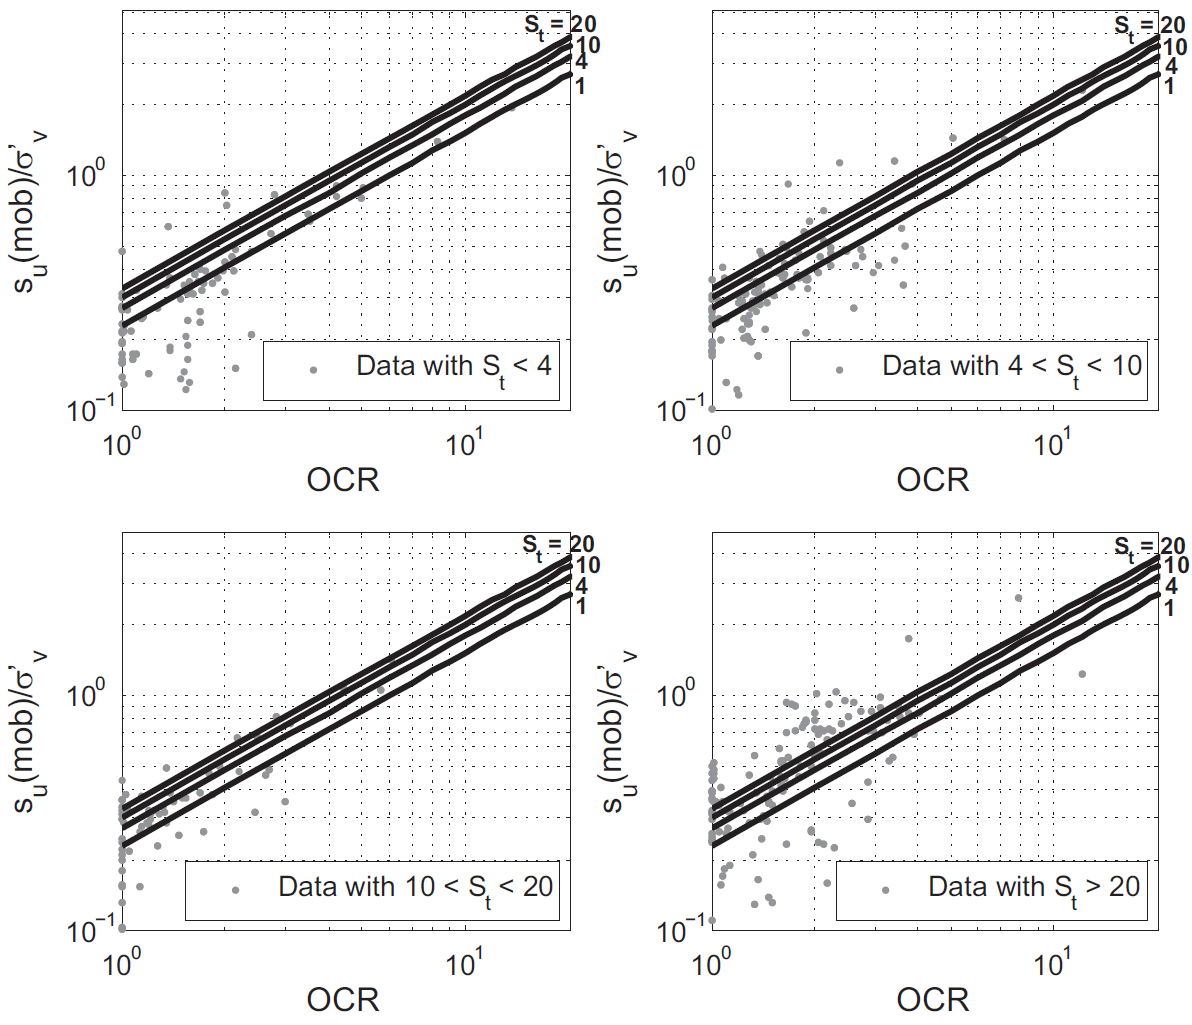
\includegraphics[width=\textwidth]{figures/figure-11.png}
        \caption{$\rm{OCR}-(s_u/\sigma_p')-S_t$ models proposed by \citet{Ching2012522}.}
        \vspace{-5pt}
        \addtocounter{figure}{-1}
        \renewcommand{\figurename}{图}
        \caption{\citet{Ching2012522}提出的$\rm{OCR}-(s_u/\sigma_p')-S_t$模型。}
        \label{figure:11}
        \renewcommand{\figurename}{Figure}
    \end{minipage}
\end{figure*}

\begin{figure*}[!p]
    \centering
    \begin{minipage}[t]{0.48\textwidth}
        \centering
        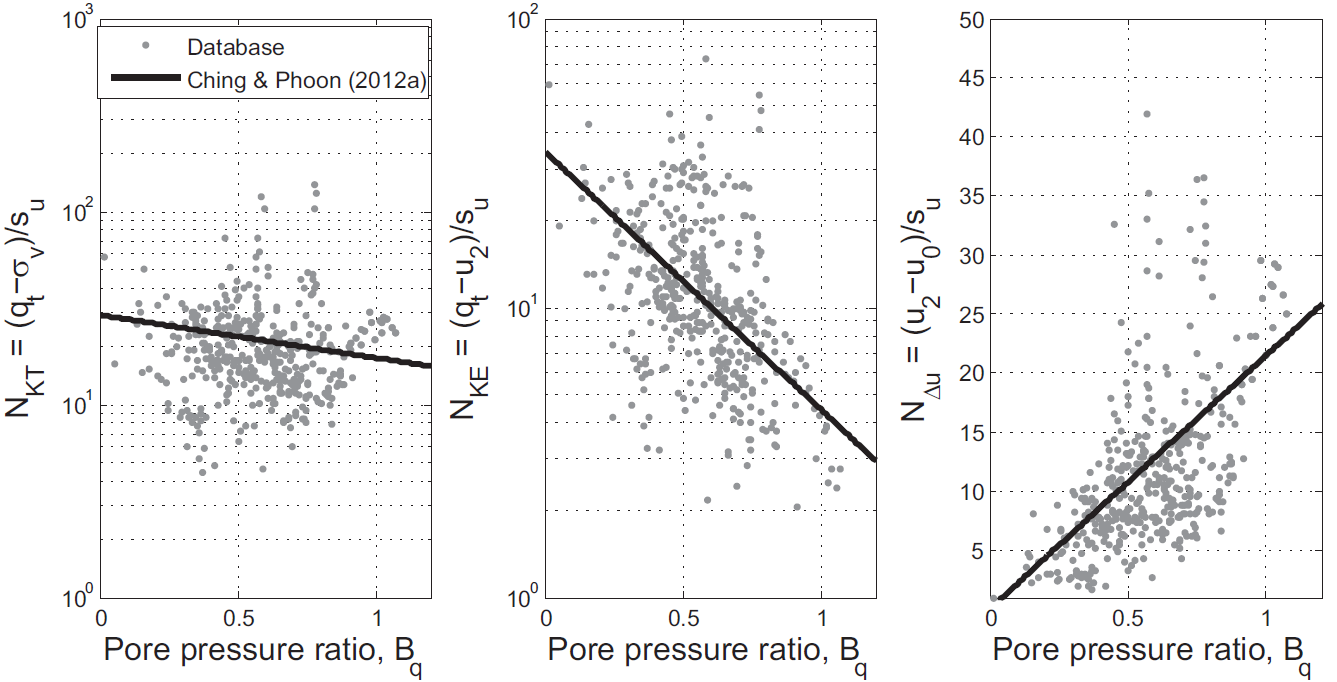
\includegraphics[width=\textwidth]{figures/figure-12.png}
        \caption{$\rm{CPTU}-s_u/\sigma_v'$ model proposed by \citet{Ching2012522}.}
        \vspace{-5pt}
        \addtocounter{figure}{-1}
        \renewcommand{\figurename}{图}
        \caption{\citet{Ching2012522}提出的$\rm{CPTU}-s_u/\sigma_v'$模型。}
        \label{figure:12}
        \renewcommand{\figurename}{Figure}
    \end{minipage}
    \begin{minipage}[t]{0.48\textwidth}
        \centering
        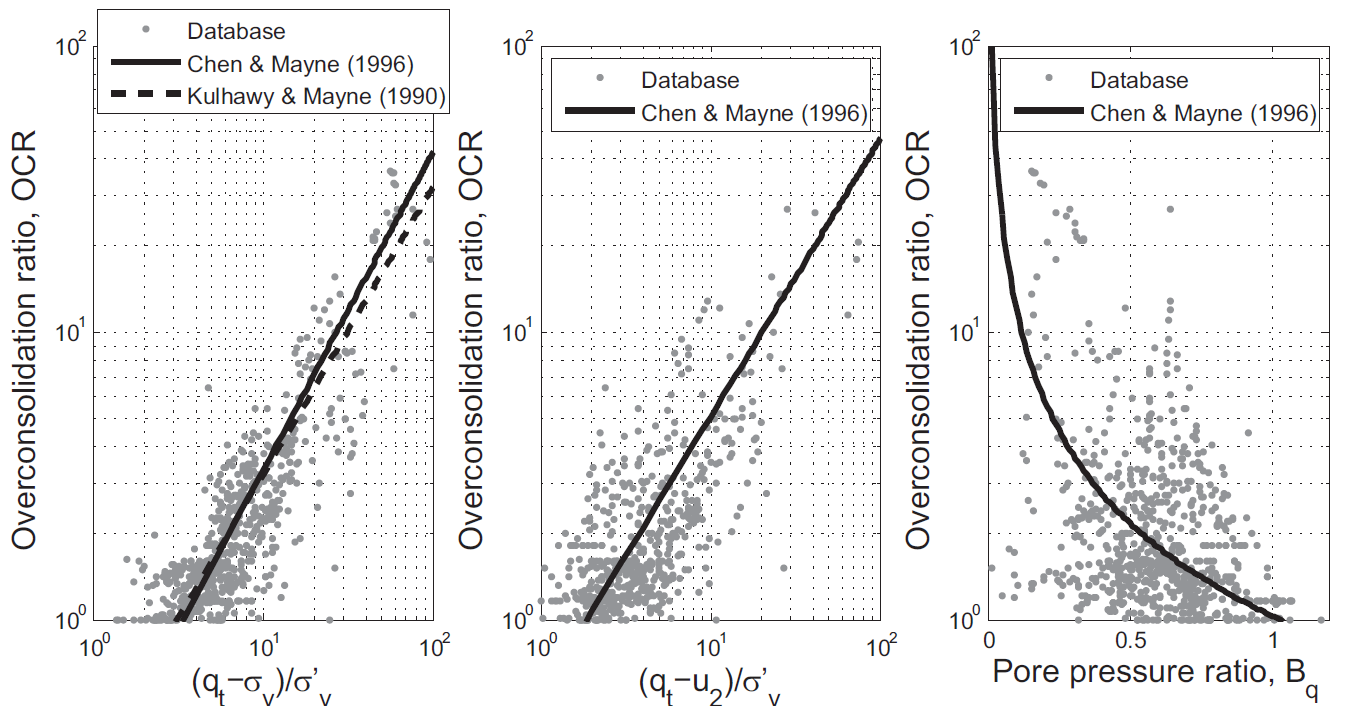
\includegraphics[width=\textwidth]{figures/figure-13.png}
        \caption{CPTU-OCR model proposed by \citet{Chen1996488, Kulhawy1990}.}
        \vspace{-5pt}
        \addtocounter{figure}{-1}
        \renewcommand{\figurename}{图}
        \caption{\citet{Chen1996488, Kulhawy1990}提出的CPTU-OCR模型。}
        \label{figure:13}
        \renewcommand{\figurename}{Figure}
    \end{minipage}
\end{figure*}

\begin{figure*}[!p]
    \centering
    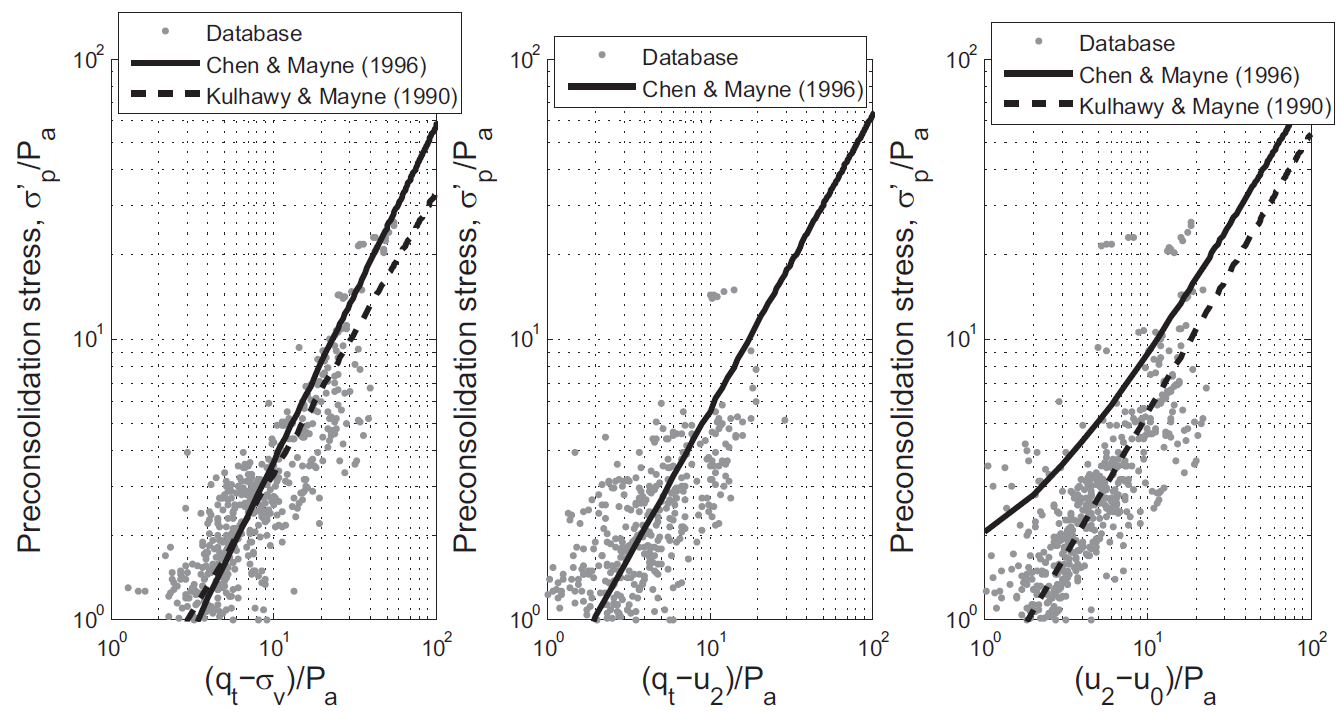
\includegraphics[width=0.5\textwidth]{figures/figure-14.png}
    \caption{$\rm{CPTU}-\sigma_p'/P_a$ model proposed by \citet{Chen1996488, Kulhawy1990}.}
    \vspace{-5pt}
    \addtocounter{figure}{-1}
    \renewcommand{\figurename}{图}
    \caption{\citet{Chen1996488, Kulhawy1990}提出的$\rm{CPTU}-\sigma_p'/P_a$模型。}
    \label{figure:14}
    \renewcommand{\figurename}{Figure}
\end{figure*}
